\ifdefined\included
\else
\setcounter{chapter}{3} %% Numéro du chapitre précédent ;)
\dominitoc
\faketableofcontents
\fi

% \chapter{Designing a Model of Collaborative Execution and its integration in a task planner}
\chapter{A Task Planner Making a Robot Compliant to Human Online Decisions and Preferences}
\chaptermark{Compliance to online human decisions and preferences}
\label{chap:4}
\minitoc


\section{Introduction}

\textit{From HRI paper}

In the context of HRC for a shared task~\cite{selvaggio2021autonomy}, we believe, based on the literature on joint action~\cite{sebanz-2006joint,sebanz-2009,clodic-2017,gordon-2023}, that the key towards a seamless interaction is, to consider the human as an uncontrollable agent and to be fully and concurrently compliant with them. 
The human should not be dictated which action they must perform, as in~\cite{roncone2017transparent,buisan:hal-03684211}, and the robot must comply with possible human decisions and actions during execution.

To collaborate with such humans with their (hidden) preferences, one can devise an online planning scheme coupled with a plan executor. 
However, in order to maintain real-time performance, online planning generally keeps a restricted horizon. 
Therefore, decisions taken online may lead to a dead end or may not lead to an optimal solution. 
Offline planning overcomes these issues. 

We propose a new \textit{offline} task planner which extends an existing human-aware planning system addressed in~\cite{buisan:hal-03684211}. 
The new planner is designed to take into account a \textit{Model of Execution}, which is in the form of an automaton and mainly inspired by the joint actions schemes. 
The model captures humans' latitude in their decisions. 
The planner's output is the robot's behavioral policy, which describes the robot's action in a state such that the action is congruent and compliant with the human's decision in this state and their (estimated) preferences, and that it is also legal to be executed in parallel. 
Our framework also allows humans to share their (new) preferences at any time during execution while the robot's policy is adapted online to that. 
In addition, our approach considers social signals to enhance execution by minimizing uncertainties. Both humans and robots issue signals to clarify situations such as performing an action, waiting for the other agent's necessary actions, or indicating a desire to remain passive.

In this chapter, we discuss relevant related work before describing the joint action model of execution that is central to our approach. 
We then describe the task planning problem and then introduce our novel framework. 
The following two sections to that, explain how the robot policy is generated by a three-step process: \textit{exploration}, \textit{characterization}, and \textit{generation}. 
We empirically evaluated our approach in simulation. With a BlocksWorld scenario, we show how our approach can effectively produce a concurrent robot behavior that is compliant with human online decisions and preferences.  


\section{Related works}

\textit{From HRI paper}

There have been a few attempts to cater to concurrent execution, but they deal with explicit time to manage concurrency~\cite{CirilloKS09a,kockemann2014grandpa}. 
In~\cite{CirilloKS09}, the robot does not plan actions for humans but forecasts their actions/plans from their activities and bases its own decision on the distribution of possible human plans. Here robots can perform actions concurrently, estimating/managing the completion time of the agents' actions carefully. 
We can see the human activity recognition part as a form of our \textit{identification (ID)} process of the automaton used. The robot needs such a plan/goal recognition technique to be compliant with the human's decisions. 
But, unlike ours, they do not consider an explicit shared goal among the agents, and hence humans are not concerned with stuff robots might be interested in during collaboration, e.g., giving signals to be passive. 
We believe that a shared goal creates a different context in HRC than the robot just being compliant with an estimated human's goals/plans. 
Moreover, we claim that dealing with concurrent actions is inevitable in planning even if actions are instantaneous, to effectively deal with multiple agent systems~\cite{CrosbyJR14,ShekharB20}, especially if there is a human operator involved like in our case. 
We extend HATP/EHDA~\cite{buisan:hal-03684211} to demonstrate that.

In another work, both \textit{recognition} and \textit{adaptation} take place simultaneously and comprehensively~\cite{levine2014concurrent}. 
It deals with action scheduling of an already generated contingent plan comprising human's and robot's actions. 
It outputs schedules for the robot actions that can execute concurrently but to do that explicit temporal constraints are considered. 

Ramachandruni, Kent, and Chernova (2023)~\cite{RAMACHANDRUNI2023} propose a communication free human-robot collaborative approach for an adaptive execution of multi-step tasks. 
In their approach, the robot observes and supports human decisions, actively selecting actions to optimize collaborative task efficiency. 
Unlike our approach, they introduce an extended collaborative HTN representation with role assignment for planning and state tracking during execution, which is more in line with~\cite{roncone2017transparent}. 
In contrast, we employ two distinct HTNs for robot and human capabilities and use an AND/OR tree for exploration and execution tracking. While their online planning may enhance scalability, optimality is not guaranteed. 
Also, our scheme accommodates both verbal and non-verbal communication, allowing the human to express preferences that update the robot policy online. 



\section{Model of Execution}

    \subsection{Rationale}



Our task planning approach uses a model of execution to improve the fluency and amenability of HRC. 
This model is in the form of an execution controller as shown in Figure~\ref{fig:model_of_execution}, and is based on several key notions and mechanisms borrowed from studies on joint actions~\cite{Sebanz-2016,kourtis2014attention}, and adapted to Human-Robot Joint Action~\cite{clodic-2017,curioni-2019}.
The key idea is that co-acting agents co-represent the shared task context and integrate task components of their co-actors into their own task representation~\cite{Schmitz-2017, Yamaguchi-19}. Also, coordination and role distribution rely strongly on reciprocal information flow, e.g., social signals~\cite{curioni-2019}, prediction of other's next action~\cite{luke-2018}.

Our proposed execution model is implemented on a robot that co-acts with a human, integrating explicit representation and exploration of the task representations for the robot and for the human. 
It also identifies precisely how reciprocal information flow is used in task execution (detecting and interpreting human actions, signals produced by the robot while acting, and also when the robot waits for human actions or their signals).

Another essential question is the criteria for choosing the next action, or more globally, how to share the load between the two co-actors. The choice depends on the context and actors' preferences~\cite{Gombolay-2015, Strachan-2020, Curioni-2022}. 
Concerning the case when one actor is a robot, we think it is important to provide a standard default behavior of the robot where the robot does its best to reduce human load but still leaves full latitude to act whenever humans want. 
Our scheme provides this ability and also allows humans to inform about their preferences at any moment.

\subsection{Simplified Model of Execution - Robot Automaton}

\begin{figure}
    \centering
    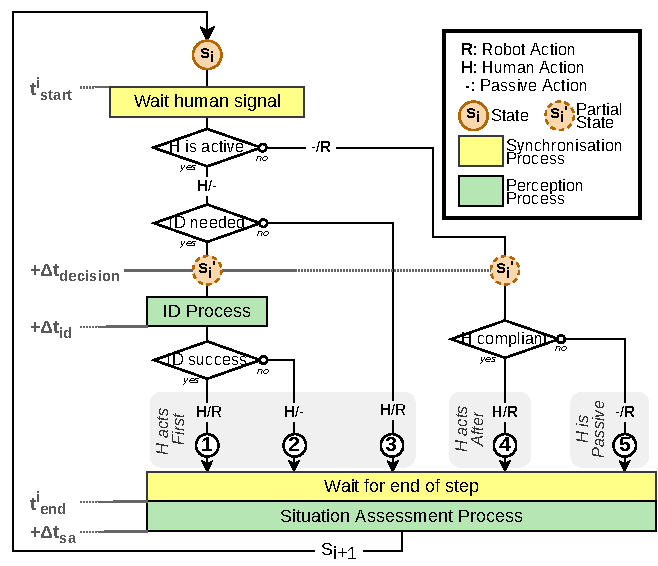
\includegraphics[width=0.8\linewidth]{Chapter4/simplified_automaton.pdf}
    \caption{
    Simplified Model of Execution in the form of an automaton run by the robot. It captures the latitude of uncontrollable humans in their actions and guides our task-planning approach.
    In this paradigm, the two agents can act concurrently but one is always compliant with the other's decision to act.
    Here, the human is always free to decide whether to start acting first, or after the robot, or not to act at all.
    To be compliant, the robot attempts to identify human decisions using perception and situation assessment as well as possible collaborative human signaling acts (e.g., gestures or speech).
    }
    \label{fig:model_of_execution}
\end{figure}

% Full page figure formats w/r line of caption:
% - 5 lines = 210x294 ratio
% - 4 lines = 210x301 ratio
% - 3 lines = 210x308 ratio


Consider an example to clarify the execution automaton. 
Assume a human and a robot have to pick up two blocks, \textit{A} and \textit{B}, that both can reach. 
They can pick it up both at the same time unless they try to pick up the same block, which causes conflicts between their actions. 
As a result, despite being executable in parallel, the actions are interdependent, and in order to avoid conflicts, one agent must be compliant with the other. 
However, if we consider a third block \textit{C} that only the robot can reach, it can always pick up this block without any risk of conflicts with the human's choice. 

In a state, a human decision can result in one of three outcomes.
First, the human can choose to act first (\textit{left~subtree}).
If the robot's best action is not in conflict with the human action (e.g., \textit{pick~C}), the robot can safely perform this action concurrently with the human operator (\textit{branch~3}).
However, if the robot's best action is either \textit{pick~A} or \textit{pick~B}, the human action must be identified first with a subroutine in order to be compliant with it.
If this subroutine is successful the robot can perform any action which is congruent with the identified human action (\textit{branch~1}). 
This includes the robot's choice to be \textit{passive} and let the human act alone. 
However, if the robot is unable to identify the human action, it must remain passive in order to avoid potential conflicts (\textit{branch~2}). 
Then, the human can either decide to be \textit{passive} or to act after the robot (\textit{right~subtree}). 
In both cases, the human is \textit{passive} at the beginning, making the robot to start performing alone a feasible action. 
While the robot is acting, the human is free to remain \textit{passive} until the next step (\textit{branch~5}) or to choose a congruent action to act concurrently (\textit{branch~4}). 
As a result, the human can always choose to 1) act first, 2) act after the robot, or 3) not act at all. 
The robot will always be compliant with these online human decisions.

When both agents finish their actions, the step is considered as \textit{``over''}. 
Then, another subroutine assesses the new world state ($s_{i+1}$), which is the result of the concurrent actions being executed in the state $s_i$, before repeating the whole process until the task is solved.

Note that if both agents are passive (the human decides to be passive when the robot cannot act) then the step is repeated. 

\subsection{Complete Model of Execution - Dual Automaton}

Now that the idea behind this model of execution has been explained we can present its complete version. Our model supposes that the robot is running an automaton to synchronize with the human, follow the generated policy, and execute actions. This automaton is a bit more complex than the simplified version presented above. Additionally, our model supposes that the human is also following an automaton when collaborating with the robot. The complete model specifies the human automaton and the visual signals exchanged between the agents to synchronize themselves.


\begin{figure}
    \centering
    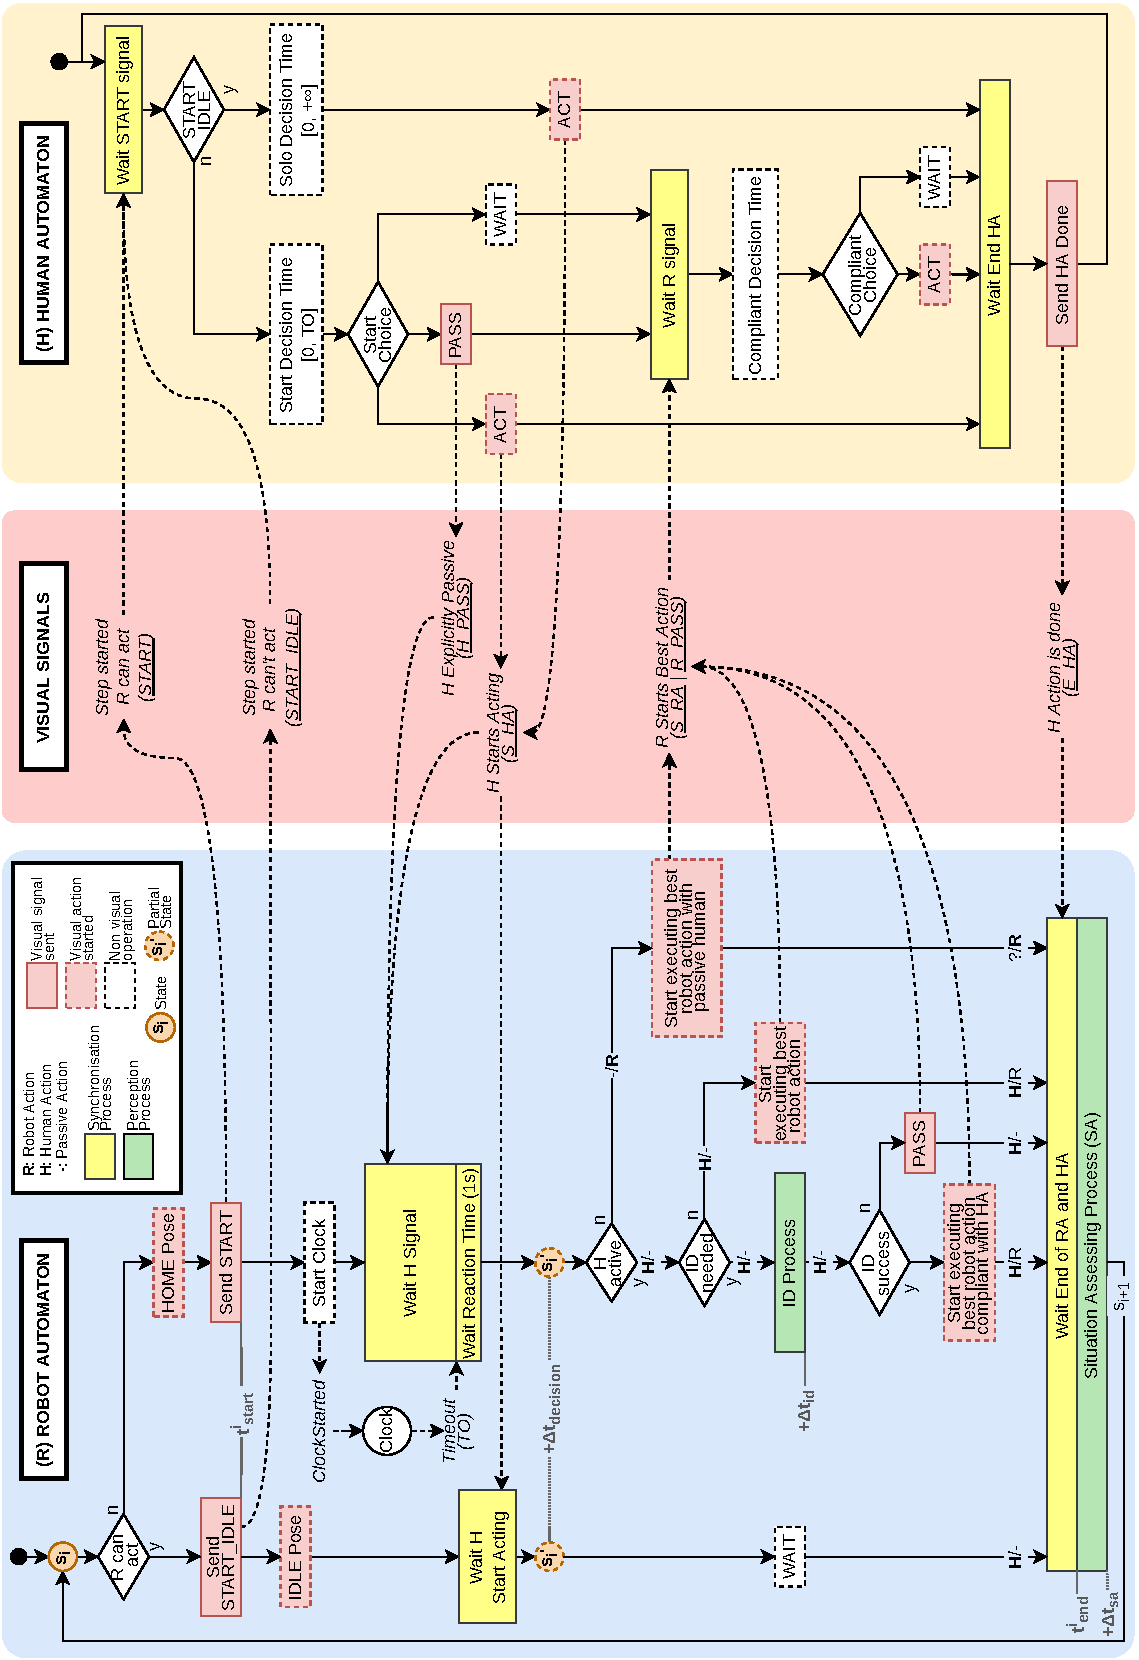
\includegraphics[width=0.99\linewidth]{Chapter4/complete_automaton_rotated.pdf}
    \caption{Complete Model of Execution - Dual Automaton. This version details the robot automaton and the assumed human automaton as well as the visual signals exchanges between the agents to synchronize themselves.}
\end{figure}

\section{Problem specification + solution}

    \subsection{Problem}

Belief divergences are out of the scope of this particular work. Hence, for simplicity reasons, we consider the two beliefs (robot and estimated human ones) as always aligned, and they are represented as a unique world state. However, we are convinced that this work could be adapted easily to consider the two distinct beliefs.

The problem is specified as follows. One initial world state, described using state variables. Distinct human and robot action models described with HTNs. Distinct human and robot initial agendas. 

[More details about each]

    \subsection{Solution}

A Planning state, referred as p-state, corresponds to a state in which the planning problem is while progressing toward a solution. A p-state contains the current world state (aligned beliefs of the agents) and the respective agenda of the human and the robot. Thus, keep in mind that p-states are very different from world states.
The initial p-state is formed using the initial human-robot agendas and the initial world state given in the problem specification. P-states are connected with each other through concurrent pairs of human-robot actions. Note that we consider passive actions, hence, there may be only one active agent in a pair if concurrent human-robot actions. A goal p-state is characterized by a world state satisfying given goal conditions and by empty agendas.
The exploration produces a directed acyclic graph, referred as the search graph, from the initial p-state to several goal p-states through sequences of concurrent action pairs. Thus, any path from the root to a leaf is a possible plan. Once the exploration done, search graph computed, another process extract the optimal robot policy from the graph. In the manner of an AND-OR tree, this policy indicates for all p-states the best concurrent robot action (OR node) to execute to be compliant with any possible human action (AND node).

\begin{figure}
    \centering
    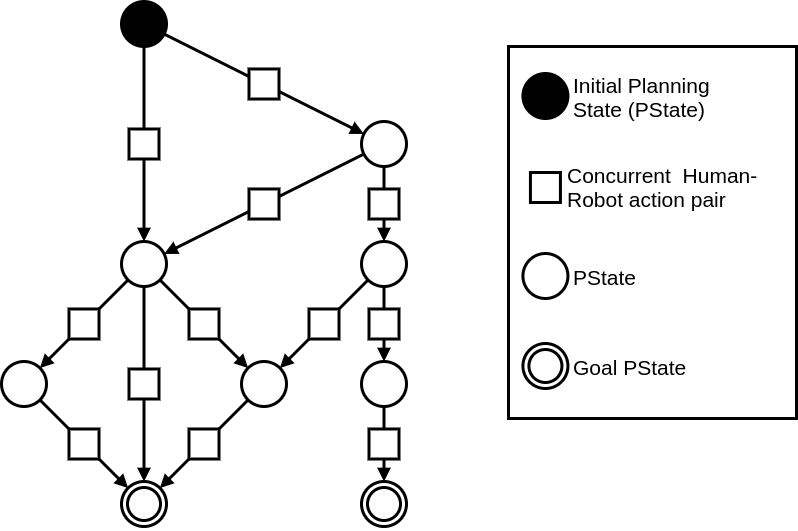
\includegraphics[width=0.7\linewidth]{Chapter4/solution_graph.png}
    \caption{Directed acyclic solution graph}
    \label{fig:solution_graph}
\end{figure}

Clarification of the directed acyclic graph. Nodes represent p-states and are connected with each other through directed edges representing human-robot concurrent action pairs. However, for practical reasons action pairs are considered as nodes of the graph having only one parent p-state node and one child p-state node. Consider that each directed edge between two p-state have one unique intermediate action pair node. The graph has one root node (no parent) which is the initial p-state. All leaf nodes (no children) represent a goal p-state. 

It is one of our design choice to do not consider explicit action costs and perform an exhaustive offline search to produce this search graph in order to solve a problem. Since the policy generation is very quick it allows generating and updating the robot policy online according to human feedbacks. 


\begin{figure}
    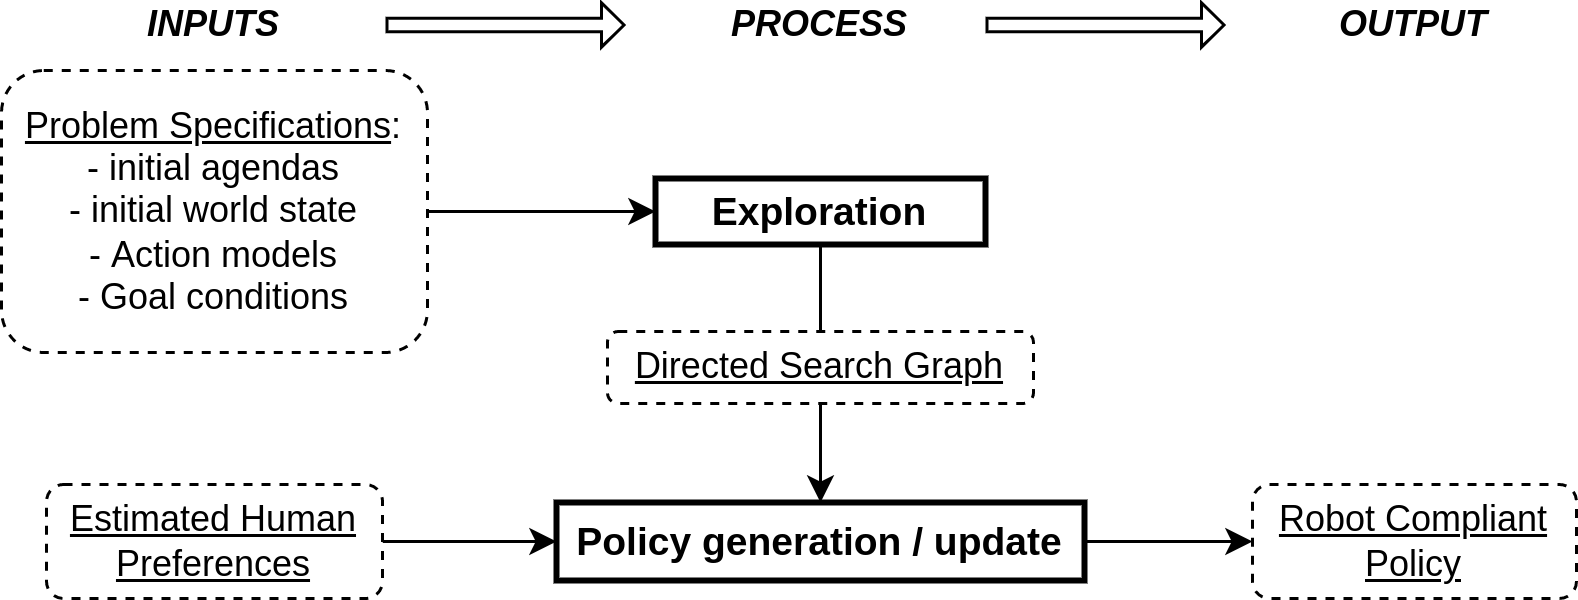
\includegraphics[width=\linewidth]{Chapter4/overall_process.png}
    \caption{Overall planning process}
    \label{fig:overall_process}
\end{figure}




\section{Exploration}

This section details how the exploration happens, and thus, how the search graph is generated. This requires several sub-process which are each detailed here. First, the overall exploration process is presented, and next subsections provide details on the sub-processes mentioned in the overall process.

    \subsection{Overall process}

We keep track of the p-state to explore, this set being initialized with the initial p-state. Then, until the set is empty we select one and explore it.
First, from this selected p-state, every possible concurrent human-robot action pairs are computed considering both agendas, the world state and reasoning on the compatibility of the actions in terms of preconditions and effects. This process requires several sub-steps and is detailed later. Thus, we obtain several action pairs leading to the same amount of new p-states (with updated world state and agendas).
Second, we check if any of the newly created p-state are similar to any existing p-state. If so, we can "merge" them to avoid redundant computations. To do so, we basically keep track of the unique p-state already checked and for each new p-state we check if it is similar to one of the already checked one. 
If not, the new p-state is added to the set of already checked p-states. 
If a similar one is found, the new p-state is deleted and the action pair leading to it is connected to the existing p-state instead.
Eventually, the remaining new p-states are added to the set of p-states to explore. 
When the set of p-states to explore is empty then the exploration is over and the graph obtained corresponds to the "search graph" where any path from the initial p-state to a leaf corresponds to a possible execution trace / plan.

    \subsection{Compute next agent actions}

From a p-state, more precisely from a world state and an agenda, we can estimate what are the next action an agent is likely to perform. Doing so is referred as the refinement process. To do so we use the corresponding action model in the form of an HTN. Here the agendas are considered as list of abstract or primitive task, where primitive task can be executed (actions), and abstract ones can be decomposed into several others subtasks. 
The refinement process consists in applying applicable methods of the first task of the agenda until it is primitive. When several methods are applicable they are all applied in a distinct refinement trace.
Eventually, for each different sequence of applied method we obtain a new agenda starting with a primitive task. For each such primitive task we create a copy of the world state contained in the given p-state, and we applied the correspond action, updating the world state. 
Hence, for each possible action a new p-state is created with the refined agent agenda, the unchanged other's agenda and the updated world state. 
Note that this process can "generate" default passive actions in several cases. First, when an agent's agenda is empty an \textit{IDLE} passive action is inserted as the first primitive task in the agenda. This means that the agent has nothing to do and thus is likely to remain passive. Either when there are no applicable methods or when the primitive task is not applicable then a \textit{WAIT} passive action is inserted. This means that the agent has still something to do but cannot do it currently. Note that when computing the concurrent pairs of action we also add the \textit{PASS} action which corresponds to the agent being voluntary passive, despite having something to do. Note also that these different passive action types just help to better understand the generated plans, but they are treated equally / similarly in the planning process.

    \subsection{Concurrent action pairs computation}

This sub-process computes from a given p-state all possible concurrent action pairs that may be executed. It is based on the previously described refinement process. This main objective of this sub-process is to identify the next actions the agents are likely to perform to reach the goal and identify which of them can be executed in parallel. The classical way to do such reasoning is by analyzing the preconditions and effects of the two actions and determine if there are conflicts between them, e.g., the effects of the first action makes the preconditions of the other false.
However, our current python implementation of the planner is convenient but has no "explicit" preconditions and effects. Everything is defined through python function. The effects of an action are a function with a world state as input and returns the updated world state. Action preconditions are functions with a world state as input and return a boolean. And methods (of an associated abstract task) are functions with world state as input and return a list of tasks to update the agenda with. Methods also have preconditions working similarly then action preconditions. 
Hence, it's challenging to extract the explicit effects and preconditions of an action. That is why we decided to rely on an assumption to check the compatibility of concurrent actions. 
We consider the following in a given state. 
If action 1 and action 2 can be sequentially performed in both orders (1$\rightarrow$2 and 2$\rightarrow$1). Then we can assume that there are no causal links between the two actions and that they can be performed concurrently. The only care to take are shared resources such as a tool that would only be used during the action, making it available before and after but not during the action. To tackle this issue, shared resources are explicitly declared in the world state and in the action models. Two actions requiring a same shared resource cannot be parallelized.
One benefit the way we check if two actions are mutually exclusive is making the actions estimations a black box. Indeed, we can easily replace the way we estimate the next actions each agent is likely to perform. Especially for the human, we could use a pretrained human activity estimator neural network, or more classical planner like PDDL. 

With the causal principle above in mind, we proceed as follows to compute the possible concurrent action pairs from a given p-state. We start by estimating all possible human actions by refining the human agenda, generating a new p-state for each possible action. For each such p-state we first create an action pair where the robot is passive by inserting a \textit{PASS} robot action. This \textit{PASS} pair is stored among all other "human pass pairs". Second, we refine the robot agenda to obtain all feasible sequences of human then robot actions and their associated p-states. We refer to them as the sequential human starting pairs. In a symmetrical way we compute the sequential robot starting pairs and "robot pass pairs" by starting with the robot then refining the human agenda.

Eventually, every action pair which is present in both the human and robot starting pairs are extracted and added to a set of concurrent action pairs. 
Additionally, here passive action are always parallelizable. Indeed, the only case where this couldn't be the case is when considering "joint actions" requiring the two agents such as lifting a table/object together. For now, such actions are not considered. Thus, the two sets of \textit{PASS} pairs are directly added to the set of concurrent action pairs. 
Lastly, a double passive pair with two PASS is generated and added to the concurrent set. This pair is special since it doesn't update the world nor the agendas, hence, it leads back to the previous p-state without progressing toward the goal. These pairs not need to be explored and help it different ways. First, it helps the execution for instance when only the human can act but decides anyway to pass voluntary. Then the policy will natively stay in the same p-state. Second, it is easy to detect dead-ends which correspond double \textit{WAIT} pairs. In such case, both agent cannot act, due to the lack preconditions for action or decomposing an abstract task, and they remain stuck without solving the task.  
Last, double \textit{IDLE} pairs indicates that both agendas are empty and thus that the task should have been solved. 

The obtained set of concurrent action pairs corresponds to all possible concurrent action that the human and the robot can execute in parallel in the initially given p-state. Each possible pair leads to a new p-state with updated agendas and world state, creating a tree structure. 

    \subsection{Merging p-states}

Although the tree structure produced by the process described above is complete and sound, it is inefficient and scales badly. Indeed, during the exploration we are likely to encounter several times similar p-states. For instance, consider an action pair where both the human and robot are active leading to a new p-state, one branch. Now, consider a first action pair where only the human is active, and a second where only the robot is active. Performing those two last pairs in both orders creates two other branches. However, even though the trace is different, the three p-states are identical (same world state and agendas) and it's highly redundant to explore independently each of them. That is why after each computation of the concurrent action pairs we check if any of the newly generated p-state is similar to an existing one, and if so, we connect the corresponding pair to the existing p-state to avoid redundant explorations. Doing so we transform the tree structure into a directed acyclic graph (on the condition that we don't consider double \textit{PASS} cycles). In the manner of a tree, we will refer to nodes without child as leaves nodes, which are goal p-states. Hence, now, each leaf can be reached with several paths. 
When looking for similar existing p-state, we assume that p-states which are parent with the new p-state, directly of not, will necessarily be different, and thus they are excluded. This speeds up the comparison process. 



\section{The Robot Policy}

First of all, as depicted in figure~\ref{fig:and_or}, all children concurrent action pairs of a p-state ($PS / ps_i$) can actually be seen as an AND-OR graph. Since we want to preserve the latitude of choice the human have at execution, each possible human choice of action is considered as an AND edge and leads to a partial p-state ($PS' / ps_i^j$). And from a partial p-state, each compliant concurrent robot action is considered as an OR edge and leads to another p-state.

Notations: A p-state is referred to as $ps$, and $ps_i$ is the $i$-th p-state. A partial p-state is referred to as $ps'$ and $ps_i^j$ is the $j$-th partial p-state of the $i$-th p-state.

Thus, generating the robot policy $\Pi$ consists in identifying the best concurrent compliant robot action $RA^*$ for each possible human action, or partial p-state $ps_i^j$.

These best concurrent robot actions are determined by aiming to optimally satisfy an estimation of the human preferences regarding the task. Eventually, at execution, the human is free to perform any of the explored action and the robot will accordingly perform an optimal concurrent action to both solve the task and satisfy their estimated preferences.

Hence, before giving more details about the policy itself, we first describe the format of human preferences, how we could estimate them, and what it allows us to do. After, we describe the actual process to generate the robot policy from the search graph using the estimated human preferences


**The robot policy consist in performing the best robot action according to the node and the human action, i.e., robot action stored in the "best compliant" pair corresponding to the human action.
If all "best compliant" pair have the same robot action, the robot can perform as soon as the step stars, otherwise the human action must be identified.**

\begin{figure}
    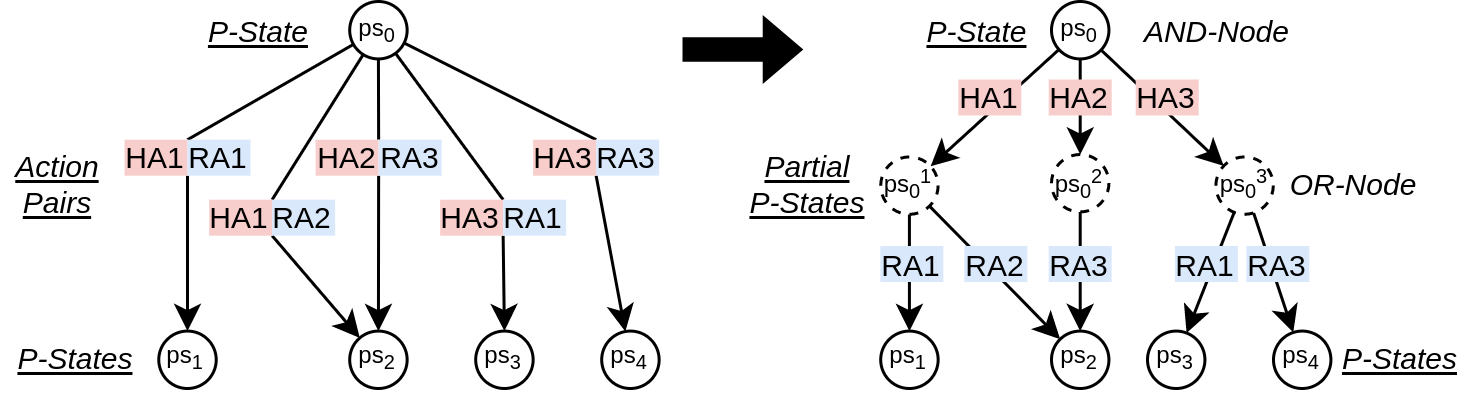
\includegraphics[width=\linewidth]{Chapter4/and_or_tree.png}
    \caption{AND-OR graph representation of the action pairs. 
    The robot policy must be compliant to any decision of the human. Hence, the problem can be seen as an AND-OR graph where for each possible human choice of action (AND node), we must determine the best concurrent robot action among the possible robot actions (OR node).
    }
    \label{fig:and_or}
\end{figure}


    \subsection{Estimated Human preferences}
estimations, format, Discussion(often inaccurate, hence our Approach), consider metrics, is a prioritized sequence of metrics to max or min, allow comparison of metrics

In this approach, instead of trying to minimize action and social costs, which are challenging to estimate accurately and quantitatively, we decided to aim at satisfying an estimation of the human preferences. In a way, the costs are included / covered / reflected in the human preferences. Our approach is to characterize each possible trace with a set of various metrics such as follows:

\begin{itemize}
    \item \textbf{Time of Task Completion}: Time step at which the task if achieved.
    \item \textbf{Time of End of Human Duty}: Time step after which the human can remain passive.
    \item \textbf{Human Effort}: Number of non-passive human action.
    \item \textbf{Global Effort}: Number of non-passive human and robot action.
    \item \textbf{*Passive While Holding}: Number of steps where an agent is passive while holding a cube.
    \item \textbf{*Number of Drop}: Number of times an agent drops cube (place back a cube on the table, not in the stack).
\end{itemize}

Note that general metrics are complemented with additional domain specific metrics (marked with a star *), given in the problem specification. The set of metrics helps to characterize and evaluate each possible plan / trace. However, even if the possible plans are characterized we so far have no way to compare them and find the best one. Doing so requires additional criteria indicating how to prioritize and compare the different metrics.

That's where we consider an estimation of the human preferences to allow us to the plans and which are given by any mean external to our system. The preferences can be estimated or also given, verbally or not. Here, we consider the human preferences in the following form. These preferences are an ordered list of the metrics characterizing the traces. Note that it's not necessary for all metrics in the list above to be present, but only them can appear in the preferences. This ordered list indicates if each metric should be maximized or minimized, and in which order / with which priority. For instance, assuming the preferences aim to minimize all metrics, the best of two given plans is the one with the lowest first metric of the list. If the two plans have equal first metric then we use the second metric, and so on. Here are two arbitrary examples of human preferences trying respectively to finish the task as fast as possible and to minimize the human effort (all metrics are minimized):

TTC - GE - HE - TEH - PWH - ND 

HE - TEH - TTC - GE - PWH - ND 

Note that estimating either human preferences or explicit action and social costs is challenging and is hardly accurate, those are very context dependent and can even vary over time.
Being aware of this, we use the estimated human preferences as a guide for the robot behavior, but we also make sure to be compliant to the human activity to lessen the impact of a wrong estimation. 

    \subsection{Generation}

\begin{figure}
    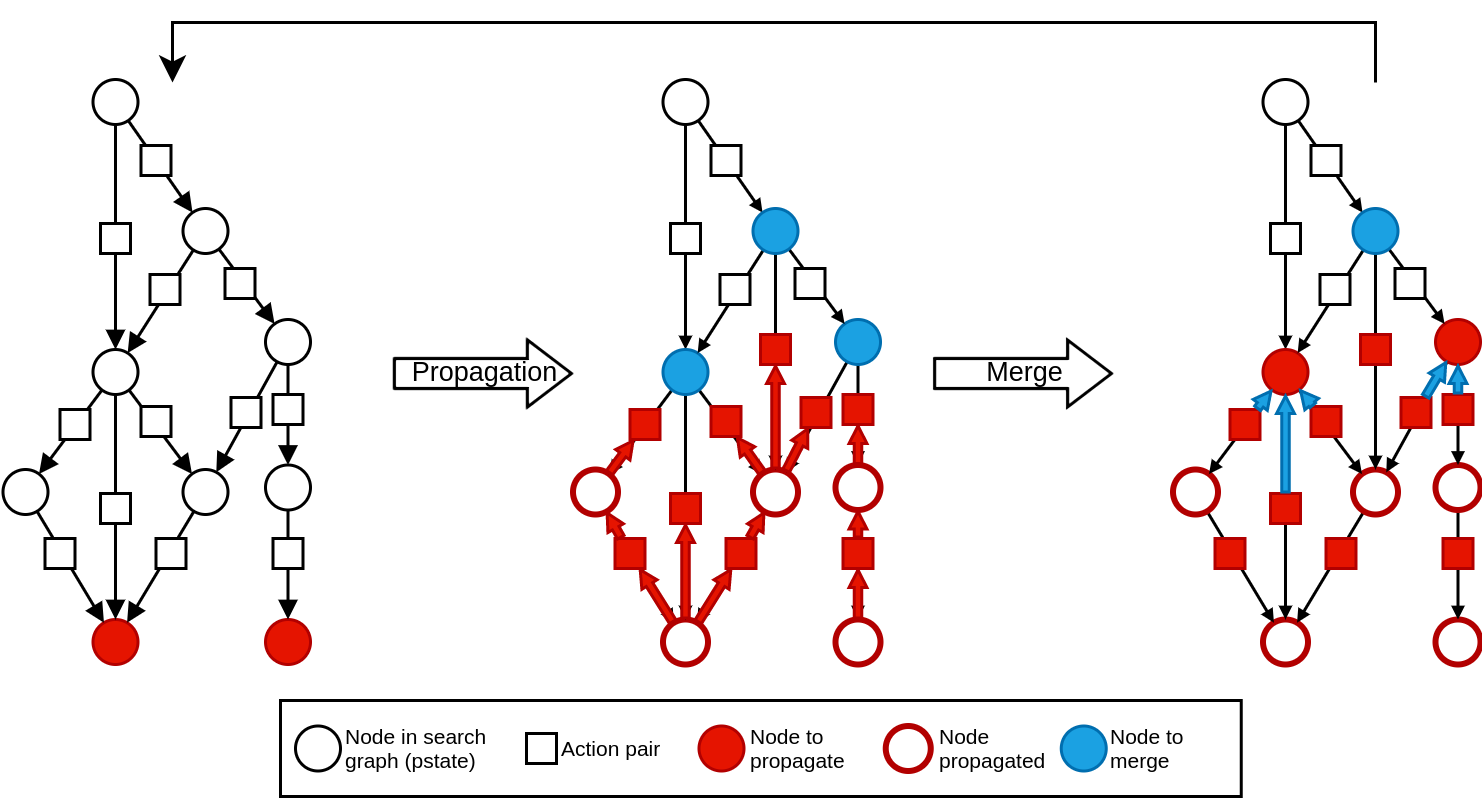
\includegraphics[width=\linewidth]{Chapter4/policy_generation.png}
    \caption{\textbf{TODO: show metrics in branches? just small $m_i$ in each branch?} Policy generation process illustration on an arbitrary search graph. Propagation and Merge processes repeat until there are no more p-state/node to propagate nor for selection.}
    \label{fig:policy_generation}
\end{figure}

To generate the robot policy $\Pi$ from the search graph we proceed from the leaves to the root. 
Overall, we progressively compute the set of metrics for each possible trace. When reaching a p-state with several children we compare the metrics of the different traces leading to this node. We are then able to identify the best trace leading to each partial p-state, and the best trace leading the p-state. Each best trace to a partial p-state is used to update the robot policy, and the overall best trace is used to continue propagation the best reachable set of metrics.
This process is achieved by repeating two sub-routines detailed just below, namely: Propagation and Selection. 

\begin{algorithm}
\caption{Policy Generation}\label{alg:policy_generation}
\begin{algorithmic}[1]

\State \textbf{input}: $leafNodes$ \Comment{Set of all leaf p-states from the search graph}
\State $psToPropagate \gets \emptyset$
\State $psForSelection \gets \emptyset$

\State $Initialization(psToPropagate, leafNodes)$

\While{ $psToPropagate \neq \emptyset$ and $psForSelection \neq \emptyset$ }
    \State $Propagation(psToPropagate, psForSelection)$
    \State $Selection(psToPropagate, psForSelection)$
\EndWhile

\end{algorithmic}
\end{algorithm}

    \subsubsection{Format and Initialization}

During this process we compute and store the best reachable set of metrics alternatively in the p-states and in the action pairs. Initially, we store default/null metrics in every leaf p-state. Then we keep track of two types of nodes. First, keep track of the nodes which metrics should be propagated in the next step, those are stored in the set $\{psToPropagate\}$ which is initialized with all leaf p-state nodes. This set is later populated by the Selection sub-routine. Secondly, we keep track of the nodes to that should select among several the best set of metrics, and thus, the best actions to perform. This set is $\{psForSelection\}$ and later is populated by the propagation sub-routine while being emptied by the selection sub-routine. The process is over when the two sets are empty, thus, when they are no more nodes either to propagate nor for selection.

% The default metrics are the following:
% \vspace{-\topsep}
% \begin{itemize}
%     \setlength\itemsep{-0.3em}
%     \item \textbf{Time of Task Completion} $= -1$
%     \item \textbf{Time of End of Human Duty} $= -1$
%     \item \textbf{Human Effort} $= 0$
%     \item \textbf{Global Effort} $= 0$
%     \item \textbf{*Passive While Holding} $= 0$
%     \item \textbf{*Number of Drop} $= 0$
% \end{itemize}

    \subsubsection{Propagation}

The propagation sub-routine is depicted in algorithm~\ref{alg:propagation} and described here. It consists in picking a node to propagate from the set $\{psToPropagate\}$. For each parent action pair of that node we create a copy of the set of metrics of the propagated node and update them according the parent action pair and propagated node. 
The metrics must be cumulative. 

Rules to update the standard metrics are the following \textbf{TODO: TO UPDATE, THERE IS AN OFFSET OF 1 FOR TIME STEP METRICS => should be done by giving the default metrics}:
\vspace{-\topsep}
\begin{itemize}
    \setlength\itemsep{-0.3em}
    \item If the pair is not \textit{IDLE}-\textit{IDLE}, then increment (by 1) \textit{Time of Task Completion}
    \item If the pair is not \textit{IDLE}-\textit{IDLE}, if the human action is passive, and if the current \textit{Human Effort} is zero, then the temporary metric \textit{Number Last Passive Human Action} is incremented.
    \item \textit{Time of End of Human Duty} = \textit{Time of Task Completion} - \textit{Number Last Passive Human Action}.
    \item If human action is not passive, then \textit{Human Effort} and \textit{Global Effort} are incremented.
    \item If robot is not passive, then \textit{Global Effort} is incremented.
\end{itemize}
Rules to updates domain specific metrics, must be provided:
\vspace{-\topsep}
\begin{itemize}
    \setlength\itemsep{-0.3em}
    \item If human action is passive and in child p-state the human is holding a cube, then \textit{Passive While Holding} is incremented.
    \item \textit{(Similarly with the robot)}
    \item If the human action is to drop a cube back on the table, then \textit{Number of Drop} is incremented.
    \item \textit{(Similarly with the robot)}
\end{itemize}

The updated metrics are stored in their corresponding action pair. Then, two cases can occur for each parent action pair with stored metrics, referred as propagated pairs. First, if the parent node of the propagated pair has more than one child then we add this parent node to the set $\{psForSelection\}$. Otherwise, the metrics of the action pair are stored in the parent node which is also added in the set $\{psToPropagate\}$. 
The sub-routine repeats until the set $\{psToPropagate\}$ is empty.

\begin{algorithm}
\caption{Propagation Sub-Routine}\label{alg:propagation}
\begin{algorithmic}[1]

\While{ $psToPropagate \neq \emptyset$ }
    \State $N \in psToPropagate$
    \State $psToPropagate \gets psToPropagate \setminus \{N\}$
    \For{ each $P$ in $N.parents$ }
        \State $P.metrics \gets CopyAndUpdateMetrics(N.metrics, N, P)$
        \If{ $HasOneChild(P.parent)$ }
            \State $P.parent.metrics \gets P.metrics$
            \State $psToPropagate \gets psToPropagate \cup \{P.parent\}$
        \Else
            \State $psForSelection \gets psForSelection \cup \{P.parent\}$
        \EndIf
    \EndFor
\EndWhile

\end{algorithmic}
\end{algorithm}



    \subsubsection{Selection}

Introduce policy notation, p-state and partial p-state (AND-OR tree)

When a node has several children, possible action pairs, then we must evaluate and compare them in order to make the best robot choices and update the policy with them. The evaluation is part is done by the propagation sub-routine. The Selection one checks when robot choices are ready to be made, update the robot policy and prepare the next propagation phase. 

The selection sub-routine is depicted in algorithm~\ref{alg:selection} and described here. It checks every node in the $\{psForSelection\}$ set to know if we are ready to make a choice, i.e., if every child pair of that node has metrics stored in it, has been propagated. 
If not, nothing happens and the node remains in the set.
If so, we are ready to compare the pairs and update the policy. Since we want the human to be free to perform any action, even suboptimal, we must find the best concurrent robot action for each possible human action. The first step is to group/sort/organize the children pairs by similar human action. Then, for each group of pairs, we compare their metrics using the estimated human preferences and identify the best pair of the group, which is marked a ``best compliant pair''. After, all marked pairs are compared the overall best pair is identified and marked as ``best pair''. Eventually, the metrics of the ``best pair'' are stored in the node from $\{psForSelection\}$, the node is removed from the set and added to the other set $\{psToPropagate\}$.

\begin{algorithm}
\caption{Selection Sub-Routine}\label{alg:selection}
\begin{algorithmic}[1]

\For{ each $PS$ in $psForSelection$ }
    \If{ $ReadyForSelection(PS)$ }
        \State $bestPairs \gets \emptyset$
        \For{ each $partialPS$ in $GetPartialPStates(PS)$ }
            \State $pairs \gets GetCorrespondingPairs(partialPS)$
            \State $P \gets IdentifyBestPair(pairs)$ \Comment{Compare metrics and identify best}
            \State $\Pi(partialPS) \gets P.robotAction$
            \State $bestPairs \gets bestPairs \cup \{P\}$
        \EndFor
        \State 
        \State $bestPair \gets IdentifyBestPair(bestPairs)$
        \State 
        \State $PS.metrics \gets bestPair.metrics$
        \State $psForSelection \gets psForSelection \setminus \{PS\}$
        \State $psToPropagate \gets psToPropagate \cup \{PS\}$
    \EndIf
\EndFor

\end{algorithmic}
\end{algorithm}

    \subsubsection{Additional policy updates}

After executing the main process to generate the robot policy $\Pi$, each partial p-state $ps'$ is mapped to a robot action to execute. So, for the robot policy to be executed the partial p-state must be identified at runtime. 
Since, a partial p-state is characterized by the choice of action the human made, this identification is done through the ID process mentioned in the Model of Execution which briefly tries to identify which action the human is starting to execute during a step. However, such identification can be challenging, so we try to avoid it when possible. 

Indeed, for any p-state $ps_i$ from the search graph, if $\forall j, \Pi(ps_i^j) = RA$ with $RA$ being one unique/same robot action, then the best robot action doesn't depend on the human choice. Thus, in such case, the ID process can be avoided, and the policy is complemented as follows $\Pi(ps_i) \gets RA$.

Moreover, we consider cases where the ID process failed to identify the human action, and is noted as $\lambda$. To prevent potential conflicts due to identification failure the policy is updated s.t. $\Pi(\lambda) = PASS$.
Note that in this work we only consider identification failures and not wrong identifications. 

% Note also that, based on the Model of Execution, each step starts when indicated by the robot, but the robot always wait for the human decision before acting. This human decision can either be active, which is easily detected, and if needed the exact human action is identified through the ID process. The human can also decide to be passive. This is detected either by observing the \textit{PASS} signal (hand gesture) or if the human neither act nor make a hand gesture within a defined time-out. Thus, for    
%% PASS always detected ?? actually not needed since not a regular action and if not identfied the TO will be triggered and it's fine. 

If human is passive ? dedicated partial p-state identified after WaitHumanDecision.

    \subsection{Execution}

The execution of the policy stems from the Model of Execution automaton and is depicted in Algorithm~\ref{alg:execution}.

\begin{algorithm}
\caption{Execution of the Robot Policy }\label{alg:execution}
\begin{algorithmic}[1]

\State $ps \gets ps_0$ \Comment{Initial state}
\While{ $ps.children \neq \emptyset$ }
    \State $IndicateStepStarted()$ \Comment{Inform the human}
    \State $WaitHumanDecision()$
    \If{ $ps \in Domain(\Pi)$ } \Comment{If ID not needed}
        \State $Execute(\Pi(ps))$
    \Else
        \If{ $HumanIsPassive()$ } \Comment{Detected by $WaitHumanDecision$}
            \State $Execute(\Pi(ps'))$
        \Else
            \State $idPartialPS \gets IDProcess()$ \Comment{$\in \{\lambda\} \cup \{ps'\}$}
            \State $Execute(\Pi(idPartialPS))$
        \EndIf
    \EndIf
    \State $WaitEndStep()$ \Comment{Human and Robot actions are done}
    \State $ps \gets AssessementProcess()$ \Comment{Identify executed pair, and next $ps$}
\EndWhile

\end{algorithmic}
\end{algorithm}

\section{Empirical Results}
simulation of execution, without durative action

We provide results obtained after simulating symbolically the execution of robot policies produced with our approach, thus without durative actions. 

    \subsection{Simulated Experiment}

The execution is symbolically simulated by running an implemented version of the automaton described in the \textit{model of execution}. This implementation is close to the presented algorithm~\ref{alg:execution} where action execution are mocked and replaced by symbolic and instantaneous actions. [Info on other mocked processes ? ID ? Wait?]
Thus, the current state progresses in the search graph based on the human decision and the produced robot policy before eventually reaching a leaf node indicating that the goal is satisfied. 
We then retrieve which course of action has been executed to then analyze it.

We evaluated our approach in the BlocksWorld domain. Figure~\ref{fig:block_world_domain} shows one problem instance. 
The human and the robot are on two sides of a big table and their shared task is to stack colored cubes as shown in the given goal pattern. 
Initially, all colored cubes are arranged on the table that is divided into three zones: Each agent has a dedicated zone (\textit{RZ} \& \textit{HZ}) and a common zone (\textit{CZ}) is in the middle and accessible for both. 
Each agent can only pick cubes from either their own zone or from \textit{CZ}. 
There is a box in \textit{RZ} in which cubes can be inserted. To pick such cubes the robot must first perform a dedicated action to open the box before being able to use the cubes inside it like the regular ones.


\begin{figure}
    \centering
    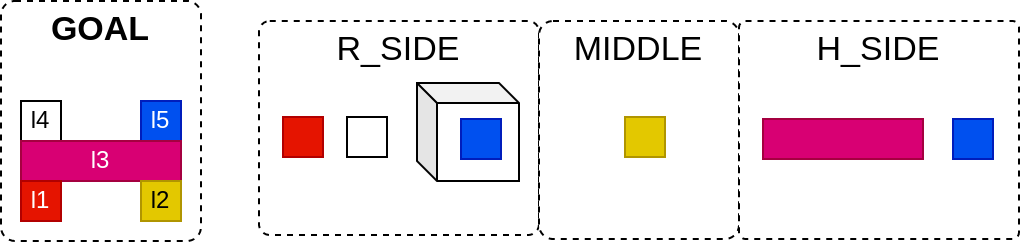
\includegraphics[width=\linewidth]{Chapter4/block_world_domain.png}
    \caption{An instance of the BlocksWorld domain. The ideal plan is strongly influenced by the human desired  preferences. For the earliest end of the task, the human prevents using the box. A lazy human will only place the required pink bar from their side. And a human in a hurry will place concurrently the yellow cube to place the pink bar at the earliest and be able to leave.}
    \label{fig:block_world_domain}
\end{figure}


    \subsection{Simulating human behavior and erroneous estimated preferences}

To simulate the human behavior, we consider and define human preferences that produce a human policy in a same manner as for the robot. The produced human policy makes the human to always perform the best action regarding their defined preferences. The robot/planner doesn't have access to the human preferences but only to an estimation of them.

In order to evaluate the quality of the executed trace regarding the actual human preferences we compare and rank every possible trace from the search graph, from best to worst. For legibility purposes we normalize the ranks to obtain a score (H-score) s.t. the trace/plan with the lowest rank has a score of 0.0, while the highest rank corresponds to a score of 1.0. This score represents a quality indicator independent of the instance's size. 
Similarly, we can do the same and acquire the score regarding the robot's estimation of the preferences (R-score). 
Keep in mind that the R-score is an estimation of the actual H-score, and the robot acts in order to maximize its R-score, hoping to maximize as well the H-score.

However, the estimation of the human preferences can be more or less accurate, causing the robot's decisions to differ from what humans would have preferred. Once again, that's why making the robot compliant with human online decisions and actions gives the human more influence over the execution and helps to reach high H-score even when the robot's estimation is incorrect.
Despite the robot trying to maximize its R-score, it's important to note that reaching a low R-score is fine as long as a high H-score is attained.

\begin{figure}
    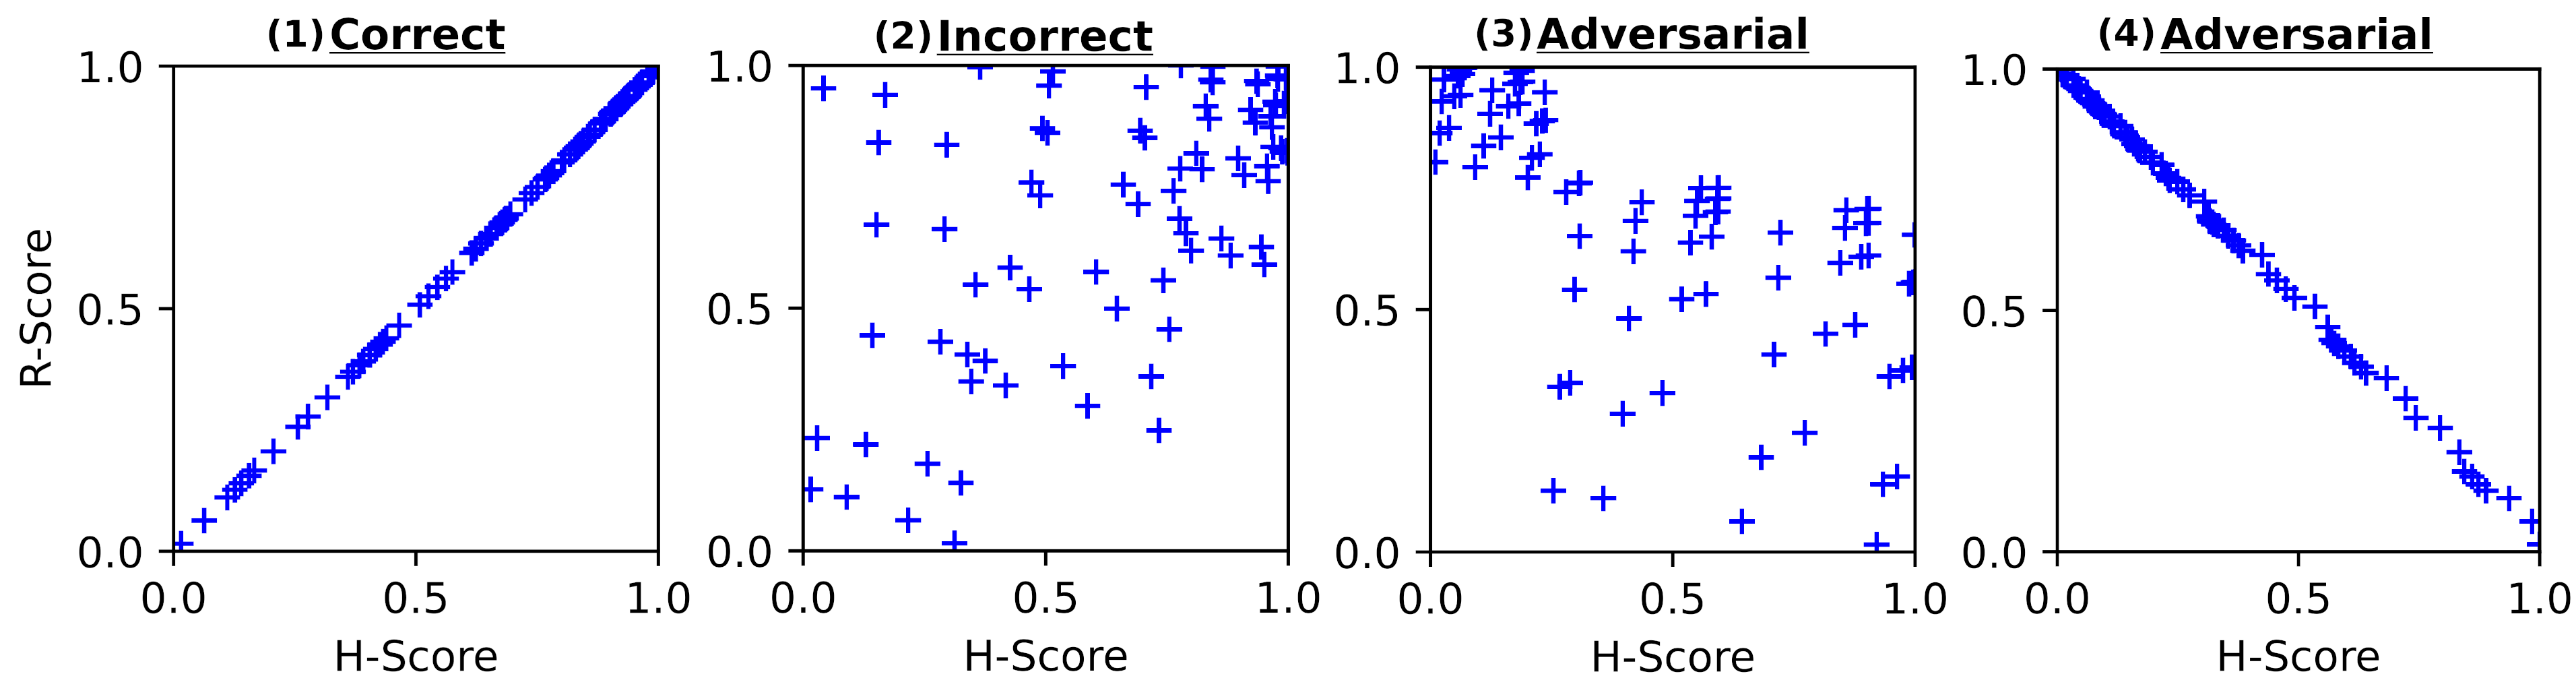
\includegraphics[width=\linewidth]{Chapter4/all_corr.png}
    \caption{
    Correlation between the H-score and R-score according to different robot estimations. Four pairs of human preferences and their estimation are considered. For each pair, all possible traces are plotted as blue crosses according their H-score and R-score. \textit{(1)} show a correct estimation while the others show incorrect estimations. \textit{(3)} and \textit{(4)} depict \textit{adversarial} estimations.
    }
    \label{fig:corr}
\end{figure}

In practice, given human preferences and their estimation creates a correlation the possibly obtained H-scores and R-scores when solving the task. Figure~\ref{fig:corr} depicts several possible correlations for a same task and same search graph but different pairs of human preferences and their estimation. On each sub figure are shown all possible traces as blue crosses according to their H-score and R-score. 
Let's consider the first case where the estimation is perfectly accurate (correct). Here, the choices of the robot which are maximizing the R-score will necessarily maximize the H-score. Indeed, when considering the few top possible robot plans (crosses with near $1.0$ R-score), the human preferences are always well satisfied (near $1.0$). 
Let's now consider the second case where the robot estimation is incorrect. Here when considering again the few top possible robot plans a wide range of H-score can be reached (near $1.0$ as well as close to $0.0$). Thus, an incorrect estimation can satisfy the human preferences but not necessarily, and so, can also fail to comply with them.
Eventually, consider the last two cases. Here, the lack of blue crosses in the top-right corners means that the H-score cannot be near $1.0$ while also having a high R-score. As a consequence, when maximizing the R-score the robot will necessarily deteriorate the quality of the plan w.r.t. the H-score. We refer to these cases as \textit{adversarial} estimations since the robot, involuntary, goes against the human will. Such cases occur when the robot estimation is far from the actual preferences and intuitively going against the latter, for instance, the robot trying to minimize the human effort while the human is actually trying to do as much as possible.  

    \subsection{Results}

\begin{figure}
    \centering
    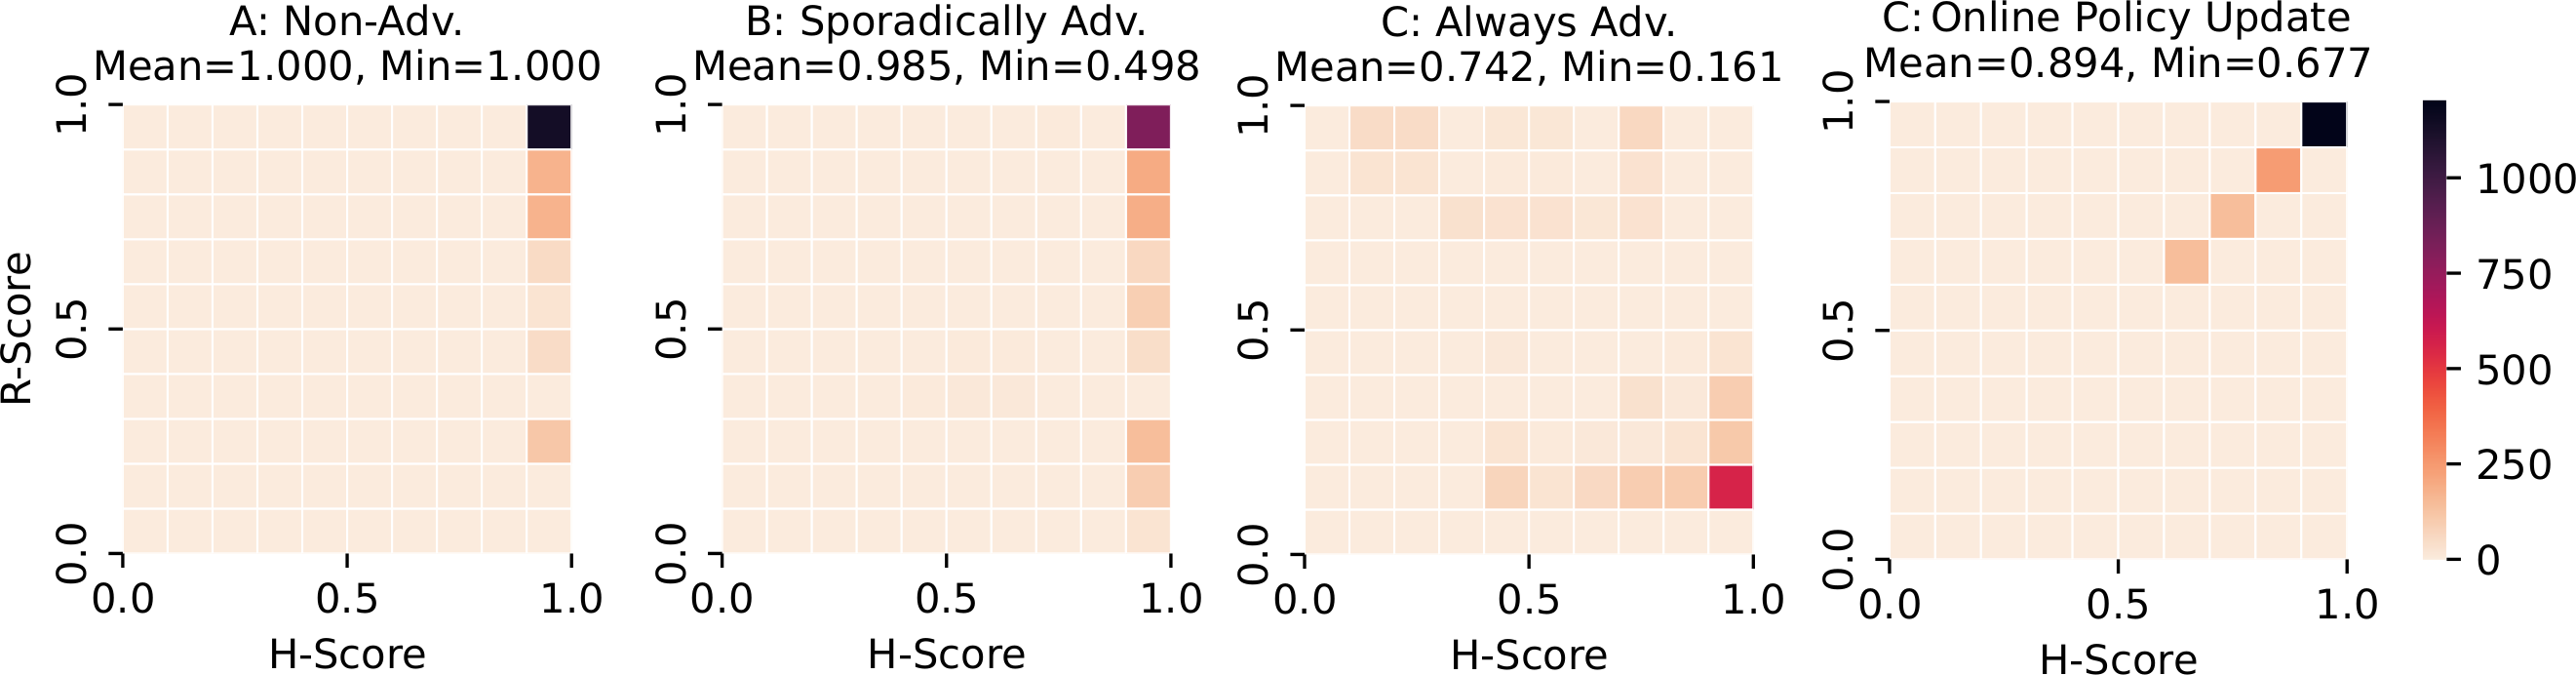
\includegraphics[width=\linewidth]{Chapter4/quant_results.png}
    \caption{
    R-scores and H-scores of the obtained executed plans after simulating the execution of the robot and the human policy generated by considering three problems and three sets of pairs of preferences/estimations. 
    The estimations in each set are (A) Never, (B) Sporadically, and (C) Always adversarial. On the right, it is shown the scores obtained using an enhanced human policy that can correct online the robot's estimation while using the set (C). \textbf{TODO: [show H mean+min and R mean+min ?]}
    }    
    \label{fig:heatmaps}
\end{figure}

For the simulations, we first generated three problems of the BlocksWorld domain with different initial states and shared tasks, and we produced for each their corresponding search graph. 
After, we generated numerous pairs of human preferences and associated robot estimation, all those pairs are categorized in three distinct sets.

In Set~A, the estimations are mostly correct and close to the human preferences (case \textit{(1)} in figure~\ref{fig:corr}). Set~B includes incorrect estimations (case \textit{(2)} in figure~\ref{fig:corr}). And Set~C contains only adversarial estimations (cases \textit{(3)} and \textit{(4)} in figure~\ref{fig:corr}).
Then, for each preference-estimation pair and each problem we generated the associated human and robot policies. Their execution was simulated symbolically using an execution automaton directly shaped upon the presented Model of Execution, and the obtained executed trace were retrieved.
The R-score and H-score of every obtained executed trace are shown as heatmaps for each distinct set of pairs in Figure~\ref{fig:heatmaps}. This will help us to highlight the benefits of using such execution scheme.

In Set~A, the estimation of the robot is close to the real human preferences and is never adversarial. So, the robot policies (maximizing the R-score) should naturally lead to high H-scores, and this is what we observed.
Some plans had an R-score lower than $1.0$ showing that the estimation was not perfect. Yet, the compliance to the human actions and the non-adversarial choices of the robot allow to always satisfy the maximal H-score of $1.0$, and thus, to always satisfy the human preferences. 
With Set~B, the incorrect estimations induced some detrimental robot choices, preventing the human from always reaching a score of $1.0$. This is depicted by the minimal H-score of $0.498$ obtained. Nonetheless, the average H-score of $0.985$ indicates that the human preferences were overall largely met.
Set~C captures the worst possible estimations inducing the robot to always make adversarial choices. This is depicted by the lower average H-score ($0.742$) and the very low minimal H-score obtained ($0.161$). 
Yet, we can notice that the average H-score is still high and that the R-score drops significantly. A low R-score means that the robot wasn't able to follow its policy correctly. Indeed, thanks to our model of execution, the robot comply to the human online decisions and purposely deviate from its ``optimal'' policy to let the human follow their own optimal policy. Eventually, the relatively high H-score obtained shows that the compliance is effective and compensates significantly (of course not totally) for a very poor estimation of human preferences. 

Additionally, we can reasonably complement the human policy, which is so far only based on preferences, with a \textit{rule}. Whenever the robot performs an action that degrades significantly the best reachable H-Score, then the human reacts by correcting online the robot estimation.
The rightmost sub-figure in Figure~\ref{fig:heatmaps} shows the new scores obtained using the Set~C and the complemented human policy. 
We notice that correcting online the estimation avoids very low human scores (minimum of $0.677$), and increases significantly the average H-score as compared with the original Set~C results (from $0.742$ to $0.894$). Hence, making the robot compliant with online preferences is very effective in improving the quality of the joint plan executed.

\textbf{TODO: [Comparison with baseline ??? ... this lack was criticized... A simple baseline with Robot first? Should show that on correct is fine but then H-score is highly degraded... Should be a mirror case of our results However, must replicate results and create more... currently unclear if can replicate.]}

Overall, we can see that the compliant robot behavior regarding both online human actions and preferences benefits the collaboration thanks to the high human scores obtained.

Consider some counter-cases from social robotics (or HA collaborative planning). Assume a robot not giving the initiative to humans always executing the best action it found. 
It is less acceptable and restricting for humans this way, even if the robot computed its best action by taking into account some social rules and estimated preferences. 
Unlike here, humans would appear compliant with the robots. 
In those cases, as it is evident from our simulation results in adversarial setups, the robot strongly impacts the solution H-score. Thus wrong robot choices can significantly degrade the human scores. In some sense, being compliant and adjusting to online preferences can be seen as some social factor that robots should maximize, and our framework helps achieve that.

\section{Performances}

\textbf{TODO: To develop...}

In this section, we provide some details about the computational performances of our approach. 

\begin{itemize}
    \item Aware that doesn't scale well
    \item HRC scenario never requires long plans (10-15 actions), restricted horizon
    \item Here clearly enough for our scenarios
    \item This already allows to explore millions of possible plans
    \item Give some numbers: Exploration time (tens of seconds, clearly ok but should be done offline) + policy generation (less than a second, can be done online) 
\end{itemize}

\section{Discussion and Limitations}

\textbf{TODO: to develop...}

\begin{itemize}
    \item Still have to synchronize with steps, currently no partial ordering. 
    \item The robot always give the initiative to the human. Should be relevant to find an in-between model of execution where the robot intelligently switch from Human-First and Robot-First, thus, sometimes taking the initiative. Either when it has no impact (robot's best action is not dependent on human choice, thus, robot could initiate the step.)
    \item Currently only symbolically simulated results, without durative actions, real humans nor real robot. Next chapter present a user study using an implemented version with durative action where a real human effectively interact with a simulated robot following the generated policy. 
    \item Assume that actions have roughly the same durations.
    \item Lack social cost, for now plan selection only relies on the estimated h preferences. Could be interesting to have a proper optimization scheme that evaluate more accurately the plans and help produce the robot policy with more criteria.
\end{itemize}


\section{Conclusion}

\textbf{TODO}




